% PREAMBLE
\documentclass[11pt]{amsart}
\usepackage[T1]{fontenc}
\usepackage{lmodern}
\usepackage{microtype}
\usepackage{amsmath,amssymb}
\usepackage{mathtools}
\usepackage{graphicx}
\usepackage{booktabs}
\usepackage{tikz}
\usepackage[colorlinks=true,linkcolor=bluedark,citecolor=bluedark,urlcolor=bluedark]{hyperref}
\usepackage[capitalize]{cleveref}

% COLORS
\definecolor{black}{HTML}{000000}
\definecolor{white}{HTML}{FFFFFF}
\definecolor{red}{HTML}{FF3D40}
\definecolor{redlight}{HTML}{FF9D95}
\definecolor{reddark}{HTML}{A80016}
\definecolor{orange}{HTML}{FF8F2C}
\definecolor{orangelight}{HTML}{FFC093}
\definecolor{orangedark}{HTML}{A25400}
\definecolor{yellow}{HTML}{FFD100}
\definecolor{yellowlight}{HTML}{FFE591}
\definecolor{yellowdark}{HTML}{9E8100}
\definecolor{green}{HTML}{32CC58}
\definecolor{greenlight}{HTML}{5EEE79}
\definecolor{greendark}{HTML}{007F2C}
\definecolor{mint}{HTML}{00D1BB}
\definecolor{mintlight}{HTML}{48EFD8}
\definecolor{mintdark}{HTML}{008173}
\definecolor{teal}{HTML}{00CAD8}
\definecolor{teallight}{HTML}{48E9F7}
\definecolor{tealdark}{HTML}{007C85}
\definecolor{cyan}{HTML}{1EC9F3}
\definecolor{cyanlight}{HTML}{86E2FF}
\definecolor{cyandark}{HTML}{007C98}
\definecolor{blue}{HTML}{008CFF}
\definecolor{bluelight}{HTML}{84BDFF}
\definecolor{bluedark}{HTML}{00559F}
\definecolor{indigo}{HTML}{6768FA}
\definecolor{indigolight}{HTML}{9EA9FF}
\definecolor{indigodark}{HTML}{3C2ABC}
\definecolor{purple}{HTML}{D332E9}
\definecolor{purplelight}{HTML}{F08AFF}
\definecolor{purpledark}{HTML}{870097}
\definecolor{pink}{HTML}{FF325A}
\definecolor{pinklight}{HTML}{FF9A9F}
\definecolor{pinkdark}{HTML}{A50030}
\definecolor{brown}{HTML}{B18462}
\definecolor{brownlight}{HTML}{DFAF8C}
\definecolor{browndark}{HTML}{754C2B}
\definecolor{gray}{HTML}{8E8E93}
\definecolor{graylight}{HTML}{BABABF}
\definecolor{graydark}{HTML}{56565A}
% COLORS END

\newtheorem{theorem}{Theorem}[section]
\newtheorem{proposition}[theorem]{Proposition}
\newtheorem{lemma}[theorem]{Lemma}
\newtheorem{corollary}[theorem]{Corollary}
\newtheorem{conjecture}[theorem]{Conjecture}
\theoremstyle{definition}
\newtheorem{definition}[theorem]{Definition}
\newtheorem{fact}[theorem]{Fact}
\theoremstyle{remark}
\newtheorem{remark}[theorem]{Remark}

\title{The Spin Spectrum Reads a Pair Census}
\author{Carlo Mitchener}
\address{MrlyProd, Inc.}
\email{carlo.mitchener@gmail.com}
\date{First published 2026-09-14}

% PAPER
\begin{document}

\begin{abstract}
Spin a black-and-white picture about its centre and record how much of it survives at each order of rotational symmetry. That list of numbers looks like a transform, but for a picture drawn as a pattern of equal square cells on a square raster it is not: every order of the list is one fixed linear function of a single table of integers, the number of filled cell pairs of each shape, two pairs having the same shape when a symmetry of the square carries one to the other. Two such pictures with the same table therefore have the same list at every order, at every resolution and under every truncation, exactly and with no transform run. At base three and one level of refinement the table has eleven entries, the designs fall into $101$ symmetry classes, and the table takes only $97$ values; the four collisions are exhibited and their spectra shown identical. Two geometric identities, a pair of cells whose rings overlap at a single radius and nowhere else and the raster's similarity to its own centre cell, pin the rank of that linear function at nine of the eleven entries, split as six even orders and three odd, and the thirteen lowest orders already attain every bound. At two levels of refinement the spectrum separates all $101$ classes with the two closest still three percent apart, so in this family the spin spectrum is a complete invariant of the symmetry class, and the credit belongs to the table.
\end{abstract}

% TITLE PAGE
\makeatletter
\global\let\titledate\@date
\global\let\paperabstract\@setabstracta
\global\let\@date\@empty
\global\let\@setabstract\relax
\makeatother

\maketitle

\begin{center}
\normalfont\footnotesize
MrlyProd, Inc.\\
\titledate
\end{center}

\vspace*{\stretch{1}}

\begin{center}

\includegraphics[width=0.8\textwidth]{figures/avatar-light.png}
\end{center}

\vspace*{\stretch{1.25}}

\newpage

\paperabstract

% BODY
\section{Introduction}
\label{sec:intro}

\begin{figure}[!ht]
\centering
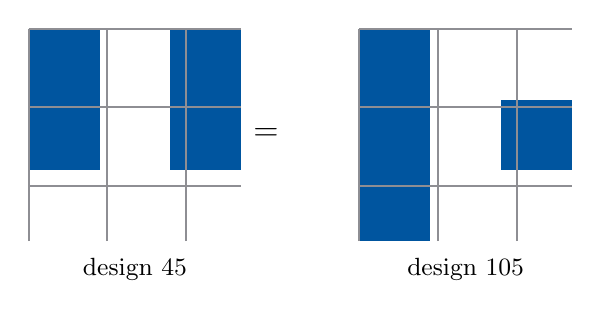
\begin{tikzpicture}[x=9mm,y=9mm]
\begin{scope}
\foreach \c/\r in {0/0,2/0,0/1,2/1} \fill[bluedark] (\c,-\r) rectangle ++(1,-1);
\draw[gray,line width=0.7pt] (0,0) grid (3,-3);
\node[anchor=north,font=\small] at (1.5,-3.1) {design $45$};
\end{scope}
\begin{scope}[xshift=42mm]
\foreach \c/\r in {0/0,0/1,2/1,0/2} \fill[bluedark] (\c,-\r) rectangle ++(1,-1);
\draw[gray,line width=0.7pt] (0,0) grid (3,-3);
\node[anchor=north,font=\small] at (1.5,-3.1) {design $105$};
\end{scope}
\node[font=\large] at (3.35,-1.5) {$=$};
\end{tikzpicture}
\caption{Two designs that no spin can tell apart at one level of refinement. They are not related by any rotation or reflection of the square and are not translates of one another, yet the eleven numbers counting their filled cell pairs class by class agree: both censuses are $(2,2,1,0,2,0,2,0,0,1,0)$. By \cref{thm:reduction} that forces every order of their spin spectra to agree exactly. Rendered one level finer they part, and \cref{fact:levels} says the spectrum then parts them too.}
\label{fig:pair}
\end{figure}

Take a black-and-white picture, spin it about its centre, and watch what the blur keeps. Turning by a third of a turn and averaging destroys everything except the part of the picture that already had threefold symmetry; averaging over every angle leaves only the part that was a set of concentric rings. Between those two extremes sits a whole ladder: for each whole number $m$, the part of the picture that repeats $m$ times around the centre, and how much of the picture's substance sits there. The list of those amounts is the picture's \emph{spin spectrum}. It is a natural thing to measure. It does not change when the picture is turned, so it is a fingerprint that survives the one transformation a spinning object is guaranteed to undergo, and it is exactly what a powder diffractometer reads off an orientation-averaged sample \cite{cherny}.

The question this paper answers is how good a fingerprint it is, and the answer is sharper and more disappointing than a transform usually allows. Draw the picture as a black-and-white pattern of equal square cells on a square raster. Then \emph{the whole spectrum is a fixed linear function of one table of integers}, and that table has nothing to do with rotation. Number the cells, and for each unordered pair of filled cells record which orbit of the square's eight symmetries that pair falls into; count the pairs in each orbit. That table of counts, the \emph{pair census}, is the only thing the spectrum sees. Two designs with the same census have the same spectrum at every order, at every resolution, under every truncation, and in exact arithmetic, no transform required (\cref{thm:reduction}).

That is not a soft statement about approximate agreement. \Cref{fig:pair} draws two nine-cell designs that are genuinely different, in different orbits of the square's symmetry group, whose eleven census numbers coincide. Their spin spectra are then equal identically, at every $m$ and at every ring resolution. There are exactly four such pairs among the $101$ symmetry classes of nine-cell designs (\cref{thm:homometric}), and they are the only obstruction at that scale: the census takes $97$ values where the classes number $101$.

Readers of crystallography will recognise the shape of this. The pair census is the Patterson function of the design, coarsened by the symmetry group of the raster, and designs with equal censuses are homometric in Patterson's sense \cite{patterson}; the classification of homometric sets is an old and hard question \cite{rosenblatt}. Readers of spectral geometry will recognise another: the question ``does the spin spectrum determine the design'' is the pattern-recognition cousin of Kac's drum \cite{kac}, whose answer in the original setting is no \cite{gordonwebbwolpert}. Readers of image analysis will recognise a third: rotation-invariant moment descriptors are old \cite{hu}, and the completeness of a truncated family of them is exactly the practical worry \cite{teague}. The contribution here is to make the reduction exact rather than approximate, to locate the loss precisely, and then to report what a complete finite search finds.

What the search finds is that the fingerprint works anyway, for a reason that is not the spectrum's doing. At base three, reading the spectrum on the level-two render of a design separates all $101$ symmetry classes of the $511$ nonempty designs, with the two closest classes still $3.3$ percent apart (\cref{fact:levels}). The reduction says this could only have happened because the two-level census separates them, and it does. So the spin spectrum is a complete invariant of the symmetry class in this family, but the credit belongs to the census, and the paper says so. And it is not the spectrum reading so many orders that nothing is left to miss: the thirteen orders used here catch at most $97.8$ percent of a design's angular energy and as little as $89.9$ percent (\cref{fact:truncation}).

The paper also measures how much of the census the spectrum throws away, and proves that the throwing-away is forced. At level one the census has eleven directions and the spectrum reads exactly nine of them. Two directions are lost, and both losses have one-line geometric causes. The centre cell of the raster lies in the closed disc of radius $\sqrt2/6$ and every corner cell in the closed region outside that disc; the two touch, and touch only on the circle $r = \sqrt2/6$ itself, which is the centre cell's farthest point and the corner cell's nearest. So a corner and the centre share exactly one ring out of a continuum, a set of measure zero, and their Gram entry vanishes at every order: one direction gone. The raster is similar to its own centre cell at ratio one third, so the spectrum of the whole square is nine times the spectrum of the centre cell at every order: a second direction gone. Those two relations cap the rank at nine (\cref{thm:rank}), and the thirteen lowest orders already reach the cap (\cref{fact:rank}). The same argument, run on the involution that half-turns one member of a pair, splits the cap into three for the odd orders and six for the even ones, and both halves are attained.

\subsection{What is proved and what is only checked}
\label{sec:roadmap}

\Cref{thm:reduction} is a theorem proved from the definitions alone, with no hypotheses beyond the ones stated: the render is a constant-valued indicator on a square raster, and the radii at which the spectrum is read do not depend on the design. \Cref{prop:classes} and \cref{thm:homometric} are finite exact statements about integers, proved by complete enumeration in integer arithmetic, \cref{prop:orbits} is proved by the orbit-counting lemma, and the reader can check the census of \cref{fig:pair} by hand in a minute. \Cref{thm:rank} is a theorem about the coefficients at every order, proved from the two geometric relations above together with the half-turn involution of \cref{lem:tau}. Everything that depends on the numerical value of a Gram entry is labelled a Fact, carries its exact finite domain, and names the script that computes it; the quadrature used is a tanh-sinh rule on an exactly located segmentation of the radius, and its agreement with a finer rule is reported alongside every number it produces.

\section{Definitions}
\label{sec:defs}

Fix a base $q \ge 2$ and a dimension $D \ge 2$. This paper is mostly about $q = 3$, $D = 2$.

\begin{definition}[design and code]
\label{def:design}
A \emph{design} is a subset $\Delta \subseteq \{0, \dots, q-1\}^D$ of the digit cells of the unit $D$-cube. Writing the cells in row-major order as $0, \dots, q^D - 1$, the design's \emph{code} is the integer $\sum_{j \in \Delta} 2^{j}$. At $q = 3$, $D = 2$ the codes run from $1$ to $511$.
\end{definition}

\begin{definition}[render]
\label{def:render}
The \emph{level-$L$ render} of $\Delta$ is the $L$-fold Kronecker power: the set $\Delta_L$ of cells of the $q^L \times \cdots \times q^L$ raster whose base-$q$ digit vectors all lie in $\Delta$. Its indicator is the function $f_L = \sum_{j \in \Delta_L} \mathbf 1_{C_j}$, where $C_j$ is the closed cell of side $q^{-L}$, on the cube $[-\tfrac12, \tfrac12]^D$ centred at the origin.
\end{definition}

\begin{definition}[spin spectrum]
\label{def:spectrum}
For $D = 2$, write a point as $(r, \varphi)$ in polar coordinates about the origin, which is the raster's centre. The \emph{$m$-th circular harmonic} of a bounded measurable $f$ is
\[
f_m(r) \;=\; \frac{1}{2\pi}\int_0^{2\pi} f(r, \varphi)\, e^{-i m \varphi}\, d\varphi ,
\]
and the \emph{spin spectrum} of $f$ is the sequence
\[
P_m(f) \;=\; \int_0^\infty |f_m(r)|^2 \, 2\pi r \, dr , \qquad m \in \mathbb Z .
\]
Since $f$ is real, $f_{-m} = \overline{f_m}$ and $P_{-m} = P_m$, so only $m \ge 0$ carries information. Parseval on each circle gives $\sum_{m \in \mathbb Z} P_m = \int f^2$, the area of the render when $f$ is a $0/1$ indicator.
\end{definition}

The name is literal. Averaging $f$ over the $q$ rotations by multiples of $2\pi/q$ kills every $f_m$ with $q \nmid m$ and keeps the rest, because the $q$-th roots of unity sum to zero; averaging over all rotations keeps $m = 0$ alone, the ring profile. So $P_m$ measures exactly how much of the design survives the rotational averaging that keeps $m$-fold symmetry.

\begin{definition}[pair census]
\label{def:census}
Let $G$ be the symmetry group of the raster fixing its centre: the dihedral group of order $8$ when $D = 2$, the group of order $48$ when $D = 3$. It permutes the $q^{LD}$ cells, hence the unordered pairs $\{j, k\}$ of cells, repetitions allowed. Let $\mathcal C_L$ be the set of orbits of that action, the \emph{pair classes}. The \emph{pair census} of any set $T$ of cells of the level-$L$ raster is the integer vector
\[
\Phi_L(T) \;=\; \bigl( \#\{ \{j,k\} \subseteq T \;:\; \{j,k\} \in c \} \bigr)_{c \in \mathcal C_L} ,
\]
and the pair census of a design $\Delta$ at level $L$ is $\Phi_L(\Delta_L)$, written $\Phi_L(\Delta)$.
\end{definition}

The pair census is a coarsening of the Patterson function \cite{patterson}: the Patterson function records the multiset of difference vectors, while $\Phi_L$ records that multiset folded by $G$ and by the raster's own boundary, so equal Patterson functions give equal censuses but not conversely. The counts are exact integers and no transform enters their computation.

\section{The spectrum is a linear functional of the census}
\label{sec:reduction}

\begin{theorem}
\label{thm:reduction}
Let $f = \sum_j x_j \mathbf 1_{C_j}$ be a constant-valued $0/1$ indicator on the cells of the level-$L$ raster, centred at the origin, with filled set $T = \{ j : x_j = 1\}$, and let $g_{m,j}$ be the $m$-th circular harmonic of $\mathbf 1_{C_j}$. Set
\[
Q_m[j,k] \;=\; \int_0^\infty \operatorname{Re}\bigl( g_{m,j}(r)\, \overline{g_{m,k}(r)} \bigr) \, 2\pi r \, dr .
\]
Then $P_m(f) = \sum_{j,k} x_j x_k\, Q_m[j,k]$, and $Q_m[\sigma j, \sigma k] = Q_m[j,k]$ for every $\sigma \in G$. Consequently $Q_m$ is constant on pair classes, and writing $Q_m(c)$ for its value on the class $c$ and $\varepsilon_c \in \{1,2\}$ for the number of ordered pairs each unordered pair of $c$ contributes, which is constant on the class because every $\sigma \in G$ carries a self-pair to a self-pair, so a class holds either only self-pairs or none,
\[
P_m(f) \;=\; \sum_{c \in \mathcal C_L} \varepsilon_c \, \Phi_L(T)[c] \, Q_m(c) .
\]
\end{theorem}

\begin{proof}
The map $f \mapsto f_m(r)$ is linear, so $f_m = \sum_j x_j g_{m,j}$ and
\[
|f_m(r)|^2 \;=\; \sum_{j,k} x_j x_k \, g_{m,j}(r) \overline{g_{m,k}(r)} .
\]
The left side is real, so the right side equals its own real part term by term after summing, and integrating against $2\pi r\,dr$ gives the quadratic form.

For the invariance, let $\rho_\theta$ be the rotation by $\theta$ about the origin. If $h = \mathbf 1_S \circ \rho_\theta^{-1}$ then $h_m(r) = e^{-im\theta} (\mathbf 1_S)_m(r)$, directly from the definition after the substitution $\varphi \mapsto \varphi - \theta$. Hence $g_{m,\rho_\theta j} = e^{-im\theta} g_{m,j}$, and the product $g_{m,\rho j}\overline{g_{m,\rho k}} = e^{-im\theta} e^{+im\theta} g_{m,j}\overline{g_{m,k}}$ is unchanged.

Now let $\sigma$ be the reflection in the line through the origin at angle $\alpha$, which sends the point $(r,\varphi)$ to the point $(r, 2\alpha - \varphi)$. Substituting $\psi = 2\alpha - \varphi$ gives $h_m(r) = e^{-2im\alpha}\, \overline{(\mathbf 1_S)_m(r)}$, using that $\overline{u_m}$ is the coefficient of $e^{+im\psi}$ for real $u$. Hence
\[
g_{m,\sigma j}\overline{g_{m,\sigma k}} = e^{-2im\alpha}\overline{g_{m,j}} \cdot e^{2im\alpha} g_{m,k} = \overline{ g_{m,j} \overline{g_{m,k}} } ,
\]
whose real part is unchanged. Every element of $G$ is one of these two kinds, so $Q_m$ is $G$-invariant, hence constant on the orbits of $G$ on pairs. Collecting the ordered pairs $(j,k)$ with both cells filled into their classes gives the last display.
\end{proof}

\begin{corollary}
\label{cor:census}
If two designs have the same level-$L$ pair census then their level-$L$ spin spectra agree exactly, at every order $m$.
\end{corollary}

\begin{remark}[rings and truncations]
\label{rem:rings}
The proof uses the radial measure only through the fact that it is the same for every cell and does not depend on the design. So the conclusion survives verbatim if $\int_0^\infty \cdot\; 2\pi r\, dr$ is replaced by a finite sum over a fixed list of radii, by a band-limited integral, or by any other design-independent radial measure. It also survives restricting $m$ to a finite set. This is why the statement is about \emph{every} ring count and \emph{every} truncation: no choice of instrument recovers what the census has already merged.
\end{remark}

\begin{remark}[three dimensions]
\label{rem:3d}
In $D = 3$ the rotation group acts on the $2l+1$ spherical harmonics of degree $l$ by an irreducible unitary representation, so a single $|f_{lm}|^2$ is not invariant and the covariant object is the total degree-$l$ power $P_l = \sum_{|m| \le l} \int |f_{lm}(r)|^2 4\pi r^2 dr$, where $f_{lm}(r)$ is the mean $\frac{1}{4\pi}\int f(r,\omega) \overline{Y_{lm}(\omega)}\, d\omega$ against harmonics normalised to $\int |Y_{lm}|^2 d\omega = 4\pi$. That is the mean-value convention of \cref{def:spectrum} one dimension up, and it keeps Parseval in the form $\sum_{l,m} \int |f_{lm}|^2 4\pi r^2 dr = \int f^2$. With that reading the proof goes through unchanged, the group being the order-$48$ symmetry group of the cubic raster.
\end{remark}

\section{Level one at base three}
\label{sec:level1}

\begin{proposition}
\label{prop:classes}
At $q = 3$, $D = 2$ the dihedral group of order $8$ has exactly $11$ orbits on the $45$ unordered pairs of the nine cells, listed in \cref{tab:classes}. At level $2$, on the $81$ cells of the $9 \times 9$ raster, it has $461$. On the $5 \times 5$ raster it has $55$ and on the $25 \times 25$ raster, one level finer at base five, $24\,805$; the order-$48$ group on the $27$ cells of the $3 \times 3 \times 3$ raster has $24$.
\end{proposition}

\begin{proof}
Direct enumeration of the orbits in exact integer arithmetic, by sweeping the pairs in order and marking each new pair's whole orbit; block 1 of \texttt{scripts/verify.py}. The level-one table is small enough to check by hand: the nine cells fall into four corners, four edge cells and one centre, so a pair is typed by the kinds of its two cells together with the distance between their centres, and \cref{tab:classes} shows that this pair of data separates the orbits and that the eleven class sizes sum to $45$.
\end{proof}

\begin{table}[!ht]
\centering
\begin{tabular}{rllr}
\toprule
$c$ & representative & the two cells & size \\
\midrule
$0$ & $\{0,0\}$ & a corner with itself & $4$ \\
$1$ & $\{0,1\}$ & a corner and a neighbouring edge cell, $\tfrac13$ apart & $8$ \\
$2$ & $\{0,2\}$ & two corners of one side, $\tfrac23$ apart & $4$ \\
$3$ & $\{0,4\}$ & a corner and the centre, $\tfrac{\sqrt2}{3}$ apart & $4$ \\
$4$ & $\{0,5\}$ & a corner and a far edge cell, $\tfrac{\sqrt5}{3}$ apart & $8$ \\
$5$ & $\{0,8\}$ & two opposite corners, $\tfrac{2\sqrt2}{3}$ apart & $2$ \\
$6$ & $\{1,1\}$ & an edge cell with itself & $4$ \\
$7$ & $\{1,3\}$ & two adjacent edge cells, $\tfrac{\sqrt2}{3}$ apart & $4$ \\
$8$ & $\{1,4\}$ & an edge cell and the centre, $\tfrac13$ apart & $4$ \\
$9$ & $\{1,7\}$ & two opposite edge cells, $\tfrac23$ apart & $2$ \\
$10$ & $\{4,4\}$ & the centre with itself & $1$ \\
\bottomrule
\end{tabular}
\caption{The eleven level-one pair classes at base three. Cells are numbered $0$ to $8$ in row-major order, so $0$, $2$, $6$, $8$ are the corners, $1$, $3$, $5$, $7$ the edge cells and $4$ the centre. Sizes are counts of unordered pairs and sum to $45$.}
\label{tab:classes}
\end{table}

\begin{proposition}
\label{prop:orbits}
The dihedral group of order $8$ has exactly $102$ orbits on the $512$ subsets of the nine cells, so $101$ nonempty designs up to symmetry, and the largest orbit has $8$ members.
\end{proposition}

\begin{proof}
The orbit-counting lemma averages the number of subsets each group element fixes, which is $2^{k}$ with $k$ the number of cycles it has on the cells. The identity has $9$ cycles; each quarter turn has one fixed cell and two $4$-cycles, so $3$; the half turn has one fixed cell and four transpositions, so $5$; each of the four reflections fixes the three cells on its axis and pairs the other six, so $6$ each. The average is
\[
\tfrac{1}{8}\left( 2^9 + 2 \cdot 2^3 + 2^5 + 4 \cdot 2^6 \right) = \tfrac{816}{8} = 102 .
\]
The empty design is one orbit, leaving $101$. The largest orbit has at most $|G| = 8$ members and attains it, for instance at the design $\{0,1\}$.
\end{proof}

\begin{theorem}
\label{thm:homometric}
The level-one pair census takes exactly $97$ values on the $101$ nonempty symmetry classes. Its four non-injective fibres each have two members, and they are the code pairs
\[
\{45, 105\}, \qquad \{61, 121\}, \qquad \{78, 102\}, \qquad \{94, 118\} ,
\]
with censuses, in the class order of \cref{tab:classes},
\[
\begin{aligned}
\Phi_1(45) = \Phi_1(105) &= (2,2,1,0,2,0,2,0,0,1,0), \\
\Phi_1(61) = \Phi_1(121) &= (2,2,1,2,2,0,2,0,2,1,1), \\
\Phi_1(78) = \Phi_1(102) &= (2,2,0,0,2,1,2,1,0,0,0), \\
\Phi_1(94) = \Phi_1(118) &= (2,2,0,2,2,1,2,1,2,0,1).
\end{aligned}
\]
By \cref{cor:census} the two members of each pair have identical level-one spin spectra at every order and every ring resolution, while lying in distinct orbits of the square's symmetry group.
\end{theorem}

\begin{proof}
The census is an integer vector computed by counting pairs, so the statement is a finite exact computation: form the $101$ canonical representatives, compute each census, and sort. Block 3 of \texttt{scripts/verify.py} does this in integer arithmetic and asserts each of the four displayed vectors. The four pairs can also be read by hand. Design $45$ is the two top corners with the two edge cells below them, design $105$ is the left column with one edge cell on the right; both have two corners and two edge cells, no centre, and the displayed census.
\end{proof}

\begin{lemma}
\label{lem:centre}
If two designs are homometric at level one and one of them avoids the centre cell, then so does the other, and adjoining the centre to both preserves homometry.
\end{lemma}

\begin{proof}
Classes $0$, $6$ and $10$ of \cref{tab:classes} are the self-pairs of a corner, of an edge cell and of the centre, so a design's census already carries its corner count, its edge count and whether it holds the centre. Homometric designs therefore agree on all three, and if one avoids the centre so does the other. Adjoining the centre adds to the census exactly the corner-centre count, which is the number of corners, the edge-centre count, which is the number of edge cells, and one in the centre-centre class. All three additions agree.
\end{proof}

Since $61 = 45 + \text{centre}$, $121 = 105 + \text{centre}$, $94 = 78 + \text{centre}$ and $118 = 102 + \text{centre}$, the four pairs of \cref{thm:homometric} are two pairs and their centre augmentations. The census counts in classes $3$, $8$ and $10$ of the augmented pairs are $2$, $2$ and $1$, exactly as \cref{lem:centre} predicts. So the four collisions are not four independent accidents but two, each doubled by a lemma that costs no hypotheses beyond homometry itself.

\section{How much of the census the spectrum reads}
\label{sec:rank}

Write $C$ for the matrix whose row $m$ is the coefficient vector $\bigl(Q_m(c)\bigr)_{c \in \mathcal C_1} \in \mathbb R^{11}$, over all $m \in \mathbb Z$. Its rank is the number of independent census directions the spin spectrum can read at level one, however many orders are used and at whatever resolution.

\begin{lemma}
\label{lem:disjoint}
$Q_m(c) = 0$ for every $m$, where $c$ is the corner-centre class.
\end{lemma}

\begin{proof}
The centre cell is $[-\tfrac16,\tfrac16]^2$, whose points are all at distance at most $\sqrt2/6$ from the origin. A corner cell, say $[\tfrac16,\tfrac12]^2$, has all its points at distance at least $\sqrt2/6$, with equality only at its single nearest corner. So for $r < \sqrt2/6$ the circle of radius $r$ misses the corner cell and $g_{m,\text{corner}}(r) = 0$, while for $r > \sqrt2/6$ it misses the centre cell and $g_{m,\text{centre}}(r) = 0$. The product vanishes off a single radius, a null set, so its integral is zero.
\end{proof}

\begin{lemma}
\label{lem:similar}
Let $o_c$ be the number of ordered pairs in the class $c$, so $(o_c)_c = (4,16,8,8,16,4,4,8,8,4,1)$ in the order of \cref{tab:classes}. Then for every $m$,
\[
\sum_{c \in \mathcal C_1} o_c \, Q_m(c) \;=\; 9\, Q_m(\text{centre-centre}) .
\]
\end{lemma}

\begin{proof}
The left side is $\sum_{j,k} Q_m[j,k]$ over all ordered pairs of cells, which by \cref{thm:reduction} is $P_m$ of the solid square $S = [-\tfrac12,\tfrac12]^2$; the right side is $9 P_m$ of the centre cell alone. The centre cell is $\tfrac13 S$, so its indicator is $\mathbf 1_S(3x)$ and its harmonics are $g_m(3r)$. Substituting $t = 3r$,
\[
P_m(\tfrac13 S) = \int_0^\infty |g_m(3r)|^2 2\pi r\, dr = \tfrac19 \int_0^\infty |g_m(t)|^2 2\pi t \, dt = \tfrac19 P_m(S) . \qedhere
\]
\end{proof}

\begin{lemma}
\label{lem:tau}
Let $\rho \in G$ be the half turn and define $\tau\{j,k\} = \{\rho j, k\}$. Then $\tau$ is a well-defined involution of $\mathcal C_1$, it fixes $5$ of the $11$ classes, it preserves $o_c$, and $Q_m \circ \tau = (-1)^m Q_m$.
\end{lemma}

\begin{proof}
$\rho$ is central in the dihedral group of order $8$, so $\{\rho(\sigma j), \sigma k\} = \sigma\{\rho j, k\}$ and the recipe descends to classes; it is well defined on the unordered pair because $\{j, \rho k\} = \rho \cdot \{\rho j, k\}$ lies in the same class. It is an involution since $\rho^2 = 1$. It lifts to the bijection $(j,k) \mapsto (\rho j, k)$ of ordered pairs, which commutes with $G$, so $o_{\tau(c)} = o_c$. Finally $\rho$ is the rotation by $\pi$, so $g_{m,\rho j} = e^{-i\pi m} g_{m,j} = (-1)^m g_{m,j}$, and $Q_m[\rho j, k] = (-1)^m Q_m[j,k]$. In the numbering of \cref{tab:classes}, $\tau$ pairs $0 \leftrightarrow 5$, $1 \leftrightarrow 4$ and $6 \leftrightarrow 9$, and fixes $2$, $3$, $7$, $8$ and $10$: five classes. Block 8 of \texttt{scripts/verify.py} recomputes the permutation and the sign rule.
\end{proof}

\begin{theorem}
\label{thm:rank}
The rank of $C$ is at most $9$. Splitting by parity, the rows of even $m$ span at most $6$ dimensions and the rows of odd $m$ at most $3$.
\end{theorem}

\begin{proof}
By \cref{lem:disjoint} the standard basis vector $e_3$ at the corner-centre class lies in the kernel of $C$, and by \cref{lem:similar} so does $u = (o_c)_c - 9 e_{10}$. At class $3$ they take the values $1$ and $8$, and at class $10$ the values $0$ and $-8$, so they are independent and the kernel has dimension at least $2$, whence rank at most $9$.

For the parity split, decompose $\mathbb R^{11} = S \oplus A$ into the $\tau$-symmetric and $\tau$-antisymmetric subspaces. \Cref{lem:tau} gives $5$ fixed classes, so $\dim S = (11+5)/2 = 8$ and $\dim A = 3$. By $Q_m \circ \tau = (-1)^m Q_m$, an even row vanishes on $A$ and an odd row vanishes on $S$, so the odd rows span at most $\dim A = 3$ dimensions. Both kernel vectors are $\tau$-invariant: $\tau$ fixes the corner-centre class so $e_3 \in S$, and $o$ is $\tau$-invariant while $e_{10}$ is fixed, so $u \in S$. The even rows therefore factor through $S / \langle e_3, u\rangle$, of dimension $8 - 2 = 6$.
\end{proof}

\begin{fact}
\label{fact:rank}
The thirteen orders $m = 0, \dots, 12$ attain every bound of \cref{thm:rank}: their coefficient matrix has rank exactly $9$, the seven even orders rank $6$ and the six odd orders rank $3$. Gaussian elimination with partial pivoting returns the same rank at every tolerance from $10^{-9}$ to $10^{-13}$, with smallest pivot $1.878 \times 10^{-4}$ against a largest coefficient of $9.806 \times 10^{-2}$. Domain: all $11$ classes, orders $0$ to $12$, level one at base three. Script: block 7 of \texttt{scripts/verify.py}.
\end{fact}

\begin{fact}
\label{fact:97}
Read on the level-one render alone, at orders $m = 0, \dots, 12$, and bucketed at tolerance $10^{-9}$, the spin spectrum splits the $511$ nonempty designs into exactly $97$ buckets, the number of census values of \cref{thm:homometric}; the four homometric pairs agree to $2.78\times10^{-17}$ on spectra of size $1.9\times10^{-1}$ to $3.0\times10^{-1}$. Domain: all $511$ codes. Script: block 9 of \texttt{scripts/verify.py}.
\end{fact}

So at level one the spectrum is strictly coarser than the census as a linear map, losing two of eleven directions, and yet induces exactly the same partition of the designs. The two lost directions are real but no design pair exploits them.

\section{What the spectrum separates}
\label{sec:separation}

One level up, the picture changes. The level-two render of a base-three design is its Kronecker square, a pattern on the $81$ cells of a $9 \times 9$ raster, and its pair census has $461$ classes instead of eleven.

\begin{fact}
\label{fact:levels}
Read on the level-two render at orders $m = 0, \dots, 12$, the spin spectrum splits the $511$ nonempty base-three designs into exactly $101$ buckets, and every bucket is a single orbit of the square's symmetry group. The largest bucket has $8$ members, matching the largest orbit. The two closest distinct classes are the designs of codes $335$ and $343$, whose spectra differ by $6.068 \times 10^{-3}$ in absolute terms and by $3.333 \times 10^{-2}$ relative to their own size, so no pair is close to colliding. Domain: all $511$ codes, orders $0$ to $12$, level two. Script: block 10 of \texttt{scripts/verify.py}.
\end{fact}

\begin{fact}
\label{fact:complete}
Within the base-three plane the spin spectrum, read on the level-two render alone, is a complete invariant of the design's symmetry class. By \cref{fact:levels} its buckets are exactly the $101$ orbits, so two designs share every $P_m$ precisely when a symmetry of the square carries one to the other, and no two designs outside a single orbit are spin-isospectral. In particular the homometry of \cref{thm:homometric} is a level-one phenomenon: the four pairs are told apart one level finer. Domain: all $511$ codes, orders $0$ to $12$, level two. Script: block 10 of \texttt{scripts/verify.py}.
\end{fact}

\Cref{thm:reduction} explains what this does and does not say. A complete invariant here is a statement about the census first and the spectrum second: the level-two census must separate the $101$ classes, or no instrument reading a rotationally averaged power could. It does, and it does so with room to spare, since it already separates the four level-one collisions in $52$, $76$, $52$ and $76$ of its $461$ class counts respectively (block 4 of \texttt{scripts/verify.py}). That the spectrum then also separates them is a second fact, and it is the one that could have failed: the spectrum sees only a rank-bounded projection of the census, and nothing in \cref{thm:rank} forbids two distinct censuses from having the same image.

\begin{fact}
\label{fact:truncation}
The thirteen orders are a genuine truncation and not a device for reading a design whole. At level one the orders $m = 0$ to $12$ hold $0.977541$ of the solid square's angular energy, against the Parseval total $\int f^2 = 1$. Over all $511$ designs that share is largest exactly at the solid square and at the lone centre cell, code $16$, where \cref{lem:similar} forces the same value, and smallest at the four one-corner designs, where it is $0.899436$. So every design spills at least $2.2$ percent of its energy into the orders the paper never reads, some spill $10$ percent, and \cref{fact:complete} separates the $101$ classes on a strict projection rather than on a complete one. Domain: all $511$ codes, orders $0$ to $12$, level one. Script: block 11 of \texttt{scripts/verify.py}.
\end{fact}

\begin{fact}
\label{fact:wider}
The census collision that would confine \cref{fact:complete} to base three does not occur elsewhere either. On the $5 \times 5$ plane the level-one census takes $3\,993\,511$ values on the $4\,211\,743$ nonempty orbits of the square's symmetry group, with $204\,856$ collisions covering $423\,088$ orbits and largest tie $8$; on the $3 \times 3 \times 3$ cubic raster, under the order-$48$ group, it takes $1\,461\,693$ values on the $2\,852\,287$ nonempty orbits, with $757\,066$ collisions covering $2\,147\,660$ orbits and largest tie $32$. Every one of those ties is broken by the level-two census, which has $24\,805$ classes on the plane and $6\,325$ in the cube; that sweep runs on a budget-capped weight window which does not bind, since it covers every tied group, all $204\,856$ of them out to weight $21$ and all $757\,066$ out to weight $24$. The canonical-form orbit counts agree with the orbit-counting averages $4\,211\,744$ and $2\,852\,288$ computed from the cycle index in the same pass. Domain: all $2^{25}$ base-five plane designs and all $2^{27}$ base-three cubic designs, and for the tie-breaking the $204\,856$ plane groups out to weight $21$ and the $757\,066$ cubic groups out to weight $24$. Script: none in this paper. The sweep runs to tens of millions of designs; it is the spin census of the MrlyMath tree \cite{tree}, whose class counts $55$, $24$ and $24\,805$ are re-derived in block 1 of \texttt{scripts/verify.py}.
\end{fact}

So $\Phi_1$ together with $\Phi_2$ is injective on symmetry classes at base three, at base five and in dimension three alike. Whether the \emph{spectrum} inherits that injectivity away from base three is open, and \cref{sec:open} says why the question is harder than it looks.

\section{Open problems}
\label{sec:open}

The paper leaves one question open above the others and it is the obvious one. \Cref{fact:complete} says that at base three the thirteen numbers $P_m$ read on the level-two render separate all $101$ symmetry classes, and \cref{fact:wider} says that the censuses $\Phi_1$ and $\Phi_2$ separate the orbits at base five and in dimension three as well. These are different statements. The spectrum is a projection of the census of rank at most $13$, acting on a census of dimension $461$ at base three and $24\,805$ at base five, and \cref{thm:rank} shows the projection already discards two of eleven directions at the smallest scale, so injectivity of the census is necessary for the spectrum to separate and is nowhere near sufficient. Does the truncated spectrum separate the orbits at base five, or in dimension three? Nobody has run the transform at those sizes, and the census result does not decide it; what is needed is either a rank argument for the level-two coefficient matrix, which this paper does not have, or a search, which at $4.2$ million orbits is a different kind of computation from anything here. Three smaller pieces of the same question are also open: whether the rank of the level-$L$ coefficient matrix has a closed form in $L$, of which \cref{thm:rank} is the case $L = 1$; whether the two relations of \cref{lem:disjoint} and \cref{lem:similar} generate the whole kernel at every level, as they do at level one; and whether a homometric pair at base three survives to level two for some larger raster, which would give a genuine spin-isospectral pair of designs and which the searches reported here say does not happen at the sizes searched.

\section{Reproducibility}
\label{sec:repro}

One script, \texttt{python3 scripts/verify.py}, plain \texttt{python3} with only the standard library, run from the paper's own directory, no arguments and no network. It takes about $2.2$ seconds and prints one labelled line per block, ending in \texttt{all green}; every check is an assertion that names the value it got, and exit code $0$ is the only pass signal.

Blocks 1 to 4 are exact integer computations and contain no floating point at all. Block 1 enumerates the pair classes of \cref{prop:classes} on the $3\times3$, $9\times9$, $5\times5$ and $25\times25$ plane rasters and on the $3\times3\times3$ cubic raster, checking $11$, $461$, $55$, $24\,805$ and $24$, the eleven class sizes of \cref{tab:classes} and their sum $45$. Block 2 checks the orbit count of \cref{prop:orbits} twice, once by the cycle-index average and once by canonicalising all $512$ subsets. Block 3 proves \cref{thm:homometric} by complete enumeration, asserts all four displayed census vectors together with the centre-augmentation structure of \cref{lem:centre}, and reads back the two cell lists drawn in \cref{fig:pair} as the codes $45$ and $105$. Block 4 computes the level-two censuses of the four homometric pairs and reports how many of the $461$ counts move.

Blocks 5 to 11 compute the Gram entries $Q_m$. The radial integral is cut at every radius where a circle can become tangent to a cell edge or pass through a cell corner, which for a raster of side $s$ is the finite set $\{\sqrt{a^2+b^2}\}$ over the half-integer grid lines, giving $5$ segments at level one and $19$ at level two; on each segment a tanh-sinh rule with $113$ nodes handles the square-root endpoint behaviour of the arc lengths. On each node the angular integral is evaluated in closed form: the circle of radius $r$ meets a cell in at most four arcs whose endpoints are exact inverse cosines and sines of the cell's edge coordinates over $r$, and $\int_\alpha^\beta e^{-im\varphi} d\varphi$ is elementary. Against a finer rule, halved in step and widened in reach, the level-one entries move by at most $6.94 \times 10^{-17}$ on entries of size up to $9.806\times 10^{-2}$, and the level-two entries by at most $8.674 \times 10^{-18}$ on entries of size up to $1.090 \times 10^{-2}$; blocks 5 and 10 print the two comparisons.

Block 5 checks \cref{thm:reduction} directly rather than assuming it: the $81$ Gram entries are computed cell by cell with no reference to the group, and the worst spread inside any of the eleven classes, over all thirteen orders, is $1.44\times10^{-17}$. Block 6 checks \cref{lem:disjoint}, which holds to the last bit because no quadrature node puts both cells on the same circle, and \cref{lem:similar} to $6.94\times10^{-18}$ cell by cell and $2.22\times10^{-16}$ in the class form the lemma states, whose eleven ordered-pair counts it also asserts. Block 7 is \cref{fact:rank}, block 8 is \cref{lem:tau} including the sign rule $Q_m \circ \tau = (-1)^m Q_m$ to $10^{-15}$ at every order, and block 9 is \cref{fact:97}, which first checks that summing $Q_m$ over the filled cell pairs of each of the $511$ designs agrees with evaluating the census formula of \cref{thm:reduction} on the same design, worst gap $3.33\times10^{-16}$. Block 10 is \cref{fact:levels}; it also recomputes the $461$ level-two coefficient vectors at a quarter-turned and at a reflected representative of each class and finds them unchanged to $1.52\times10^{-18}$, which is \cref{thm:reduction} again on the larger raster. Those two maps generate the whole group of order $8$, and the block checks that they do, so the invariance is tested across the group and not only across the rotations. Block 11 is \cref{fact:truncation}: it reads the share of angular energy the thirteen orders hold, for the solid square and for every one of the $511$ designs, so the completeness of \cref{fact:complete} is not an artefact of using enough orders to see everything.

A second script, \texttt{python3 scripts/figure.py}, draws the four homometric pairs with their shared level-one censuses and their level-two separations into the file \texttt{figures/homometric.svg}, re-checking the class tables it draws against.

One thing in this paper is outside the scripts' reach and is labelled where it appears. \Cref{fact:wider} is a sweep of $2^{25}$ and $2^{27}$ designs run elsewhere \cite{tree}; only its class counts $55$, $24$ and $24\,805$ are re-derived here. Everything else is either proved in this paper or asserted by \texttt{scripts/verify.py} on the exact finite domain stated in its own statement. The manuscript builds with \texttt{tectonic paper.tex}.

\section*{Acknowledgments}

This paper was developed and verified in collaboration with Claude (Anthropic): the proofs were drafted and checked in dialogue with the model, and the verification script and figure script were written the same way. The author takes sole responsibility for every claim.

% REFERENCES

\begin{thebibliography}{9}

\bibitem{cherny}
A.~Yu. Cherny, E.~M. Anitas, V.~A. Osipov and A.~I. Kuklin, \emph{Deterministic fractals: extracting additional information from small-angle scattering data}, Phys. Rev. E \textbf{84} (2011), 036203. \url{https://doi.org/10.1103/PhysRevE.84.036203}

\bibitem{gordonwebbwolpert}
C.~Gordon, D.~L. Webb and S.~Wolpert, \emph{One cannot hear the shape of a drum}, Bull. Amer. Math. Soc. (N.S.) \textbf{27} (1992), no.~1, 134--138. \url{https://doi.org/10.1090/S0273-0979-1992-00289-6}

\bibitem{hu}
M.-K. Hu, \emph{Visual pattern recognition by moment invariants}, IRE Trans. Inform. Theory \textbf{8} (1962), no.~2, 179--187. \url{https://doi.org/10.1109/TIT.1962.1057692}

\bibitem{kac}
M.~Kac, \emph{Can one hear the shape of a drum?}, Amer. Math. Monthly \textbf{73} (1966), no.~4, 1--23. \url{https://doi.org/10.2307/2313748}

\bibitem{patterson}
A.~L. Patterson, \emph{Ambiguities in the X-ray analysis of crystal structures}, Phys. Rev. \textbf{65} (1944), 195--201. \url{https://doi.org/10.1103/PhysRev.65.195}

\bibitem{rosenblatt}
J.~Rosenblatt and P.~D. Seymour, \emph{The structure of homometric sets}, SIAM J. Algebraic Discrete Methods \textbf{3} (1982), 343--350. \url{https://doi.org/10.1137/0603035}

\bibitem{teague}
M.~R. Teague, \emph{Image analysis via the general theory of moments}, J. Opt. Soc. Amer. \textbf{70} (1980), no.~8, 920--930. \url{https://doi.org/10.1364/JOSA.70.000920}

\bibitem{tree}
MrlyMath, \emph{the spin page and its census}, MrlyProd, Inc. \url{https://github.com/mrlyprod/mrlyprod/blob/main/research/spin.md}

\end{thebibliography}

\end{document}
